\epigraph{\textit{"It's so easy, can't you see the shift?"}}

\myparagraph{Abstract} In perovskite solar cells, the absorber is usually sandwiched between two different contacts: the \gls{htm} and the \gls{etm} with the role of extracting respectively the holes and the electrons. Without this asymmetrical extraction of charges, the photogeneration would be of no use. The classical \gls{etm} from \gls{dssc}, mesoporous titania, is slowly getting replaced by planar tin oxideCITE JIANG2018. On the contrary, the classical \gls{htm} from solid-state \gls{dssc}, \spiro, is still present in most of the record structures. The huge explorative work done for finding a more performing \gls{htm} had some success with a few molecules and, for some cases, with \gls{ptaa}. In most of the cases, even if the performances are at par with \spiro, the price is still too high for wide area applications. A better understanding of the \gls{htm}/perovskite interaction is needed for pinpointing the key characteristics to be looked for in the next \gls{htm} design. In this chapter, the devices fabricated using four different \gls{htm} have been compared in order to find a correlation with the \gls{htm}'s chemical properties.

\myparagraph{Publications} Part of this chapter has been published in %\fullcite{}.


\section{Interpretation of \gls{voc} from Current-Voltage Sweeps}


\section{Interpretation of \gls{voc} and \gls{jsc} Dependence on Light Intensity}\label{interpretation_lightintensity}

The \gls{jsc} dependency on the light intensity $\phi$ is close to linear and can be fitted with a power law $J_{SC} \propto \phi^\alpha$ as described in \cpageref{methods_jsc_intensity}. An $\alpha$ value lower than 1 indicates the presence of non-geminate recombination at short circuit\cite{Credgington2011}. Non-geminate recombination refers to the annihilation of two opposite free charges happening after their complete separation, as opposed to geminate recombination where the recombination happens just after the charges separation but before their distancing.


The \gls{voc} dependency on the light intensity $\phi$ can be fitted with a natural logarithmic dependence as described in \cpageref{methods_voc_intensity} obtaining the ideality factor $n_{id}$. This method was applied by \authoryear{Pockett2015} obtaining ideality factors as high as 5. According to \authoryear{Calado2018b}, the so-obtained ideality factor is XXXXXXXXXXXXXXXXXXXXXXXXXXXXXXXX


\section{Interpretation of Charge Extraction}\label{interpretation_ce}
\myparagraph{\Acr{ce} time constant}
The free charges extraction time is related to the RC time of the \SI{50}{\ohm} resistor and the capacitance of the solar cell device. We can see in \cref{fig:chargeExtraction_RCtime} a weak covariance (Pearson correlation coefficient of 0.3) between the RC time obtained considering the dark capacitance from \acr{dc} (geometric capacitance) and the extraction time (as obtained by an exponential fitting to a single \acr{ce} current decay) at low light intensity (enough for having a signal but far from 1~sun light intensity). At higher light intensities, the correlation is weaker as the capacitance is less defined as the cell is in a transition between illuminated (high capacitance) and dark (low capacitance) status. Anyway, the extraction time does not change much between low light intensity and 1~sun with an increase from \SIrange{1.1}{2.4}{times} (first and third quartile).

\begin{SCfigure}%[!hbtp]%
	\centering
	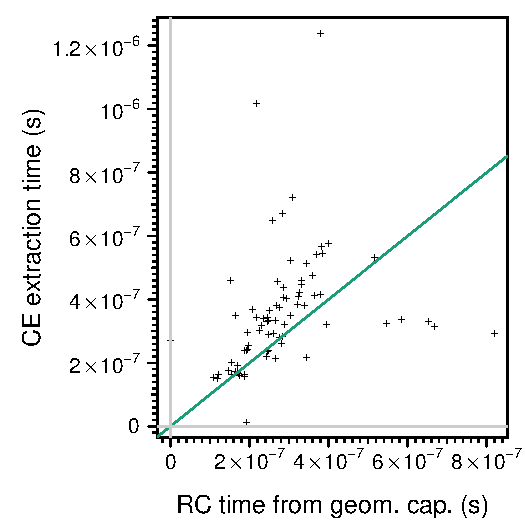
\includegraphics[width=0.45\textwidth]{chargeExtraction_RCtime/CEaBitOfSunExpTime_vs_RCdarkTime.pdf}
	\mycaption[Charge extraction time is related to a RC time.]{Covariance of \acr{ce} extraction time at low light intensity versus the expected time from geometric capacitance (as obtained from dark \acr{dc}). Each point is a different device, many different structures studied during my PhD are represented. The grey line indicates the 1 to 1 relationship.}\label{fig:chargeExtraction_RCtime}
\end{SCfigure}

\myparagraph{Comparison between \acr{ce} time constant and \acr{tpv} time constant}
During this time, and depending on its location in the device stack, some free charge can recombine. One could argue that a \acr{ce} measurement is valid only if the extraction is faster than the recombination time as measured via \acr{tpv}CITE RYAN2017 or that the extracted charge should be corrected considering the recombination CITE Credgington2011. Considering the charges accumulated in the depletion layers in the selective contacts, these will flow to the electrodes without crossing the perovskite/selective contacts interfaces, where has been reported that most of the recombination occurs CITE 10.1021/jz501163r CITE Stolterfoht2018a CITE Stolterfoht2018. So this part of the extracted charge, distinguishable as the linear part of the charge versus voltage plot, as represented in \cref{fig:} should not be corrected. Instead, regarding the charge accumulating in the perovskite layer, which we assume can be assigned to a chemical capacitance and can be recognized as the exponential part in \cref{fig:}, it may be that a correction is needed, but this has not be done in this thesis.

\myparagraph{Interpretation of the single measurement}
From some preliminary and unpublished simulations of \acr{ce} show that a short living exponential decay can be accounted for free charges and a long living and weak exponential decay is caused by a displacement current due to ionic profile updating to the new voltage. The slow decay is not usually measured and seldom reported\cite{ORegan2015b}.

\myparagraph{Interpretation of the charge versus light bias trend}


\section{Interpretation of Transient PhotoVoltage}\label{interpretation_tpv}

\myparagraph{Factors Affecting the \acr{tpv}}
The decays we can observe are limited at long times by the discharge of the extra charge through the oscilloscope resistance and through the device shunt resistance, whatever is the smallest. This happens with an RC time of the circuit composed by the capacitance of the device and the \SI{1}{\Mohm} resistance of the oscilloscope or the internal device resistance. The oscilloscope resistance could be varied using an attenuating probe (usually 10X or 100X). This limit to long times is often observed at low light intensities as a plateau in the \acr{tpv} graph. XXXXXXXXXXXXXXXXXXXXXXXXXXXXXXXXXXXXXXXXXXXXXXXXXXXXXXXXXXXXXXXXXXXXXXXXXXXXXXXXX

\begin{SCfigure}
	\centering
	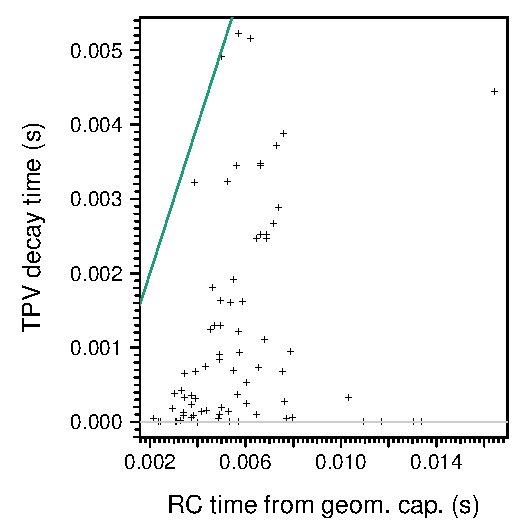
\includegraphics[width=0.45\textwidth]{tpv_RCtime/TPVdarkTime_vs_RCdarkTime.pdf}
	\mycaption[\gls{tpv} time has an upper bond due to discharge through oscilloscope.]{The green line indicates the 1 to 1 relation between the dark \acr{tpv} time (from a robust exponential fit) and the RC time derived from the geometric capacitance from \acr{dc} and the \SI{1}{\Mohm} of the oscilloscope. Each point is a different device.}\label{fig:tpv_RCtime}
\end{SCfigure}

\section{Interpretation of Transient PhotoVoltage Referenced to Charge Extraction}\label{interpretation_tpvce}

\section{Interpretation of Kelvin Probe Force Microscopy}\label{interpretation_kpfm}

\section{Interpretation of Band Gap Values Obtained via Tauc Plot, PhotoLuminescence and Computational Simulations}\label{interpretation_bg}



\section{Recombination analysis via TPV}
\section{Stored charge profile via DC}
\section{Layers workfunction via KPFM}
\section{Conclusions}
\section{Critical Assessment}